
\documentclass[12pt,a4paper,titlepage]{article}
\usepackage{amsmath}
\usepackage{latexsym}
\usepackage{amssymb}
\usepackage{amstext}
\usepackage{nccmath}
\usepackage{mathtools}
\usepackage{array}
\usepackage{fixmath}
\usepackage{mathrsfs}
\usepackage{pdfpages}

\setlength{\textwidth}{15cm} \setcounter{page}{159}

\begin{document}


\begin{titlepage}
    \begin{center}
        \vspace*{3.5cm}
        
        \textbf{\huge{Programming Assignment}}
        \vspace{1cm}

        \textbf{\huge{Report}}

        \vspace{6cm}

        \begin{verse}
            \ \ \ \ \ \ \ \ \ \ \ \ \ \ \ \ \ \ \ \ \ \ \ \ \ \textbf{\large{Student: Zhiwei Han}}\\
            \ \ \ \ \ \ \ \ \ \ \ \ \ \ \ \ \ \ \ \ \ \ \ \ \ \textbf{\large{Matrikel Nr. 03672554
            }}\\
        \end{verse}


        
        \vspace{1cm}
        
%        \includegraphics[width=0.4\textwidth]{university} 
        
        Lehrstuhl f\"ur Datenverarbeitung\\
        Technische Universt\"at M\"unchen\\
        \today
        
    \end{center}
\end{titlepage}



\setlength{\parindent}{0pt} \setlength{\parskip}{2ex plus 0.5ex
minus 0.2ex}


\section*{1. Solution with Dynamic Programming}
\subsection*{1.1 Find a mapping to linearize the state space into a vector}
The mapping is just to vectorize the 2D maze coordinates with a sparse vector and ignore the illegal states (wall grids).
\subsection*{1.2 Visualize the optimal policy with a 2d plot, where colored boxes indicate the direction of the optimal action}
In order to optimize the visualization, legal states (not a wall or out of range) are denoted as starting points with arrows instead of color boxes, and the actions are denoted as arrows. The illegal states (walls) are marked with blue squares. \textbf{The correct policy is the one in forth column of attachment 1.}\\
(The Policies please see attachment 1 and a color boxes version value function see attachment 4.)
\subsection*{1.3 Do the two methods generate the same policy?}
Yes, from the graphs in forth colomn showed in attachment 1 we know, that the policies derived from value iteration and policy iteration, are same and optimal after converge.

\section*{2. A Study of Algorithm Properties}
\subsection*{2.1 Vary the discounting factor $\alpha$. Does this have a influence on the final policy?}
Yes, discount factor $\alpha$ decides how further the algorithm looks into future. If it is too small, the algorithms cares only about the step reward instead of next state value function and hence only the states near the goal state can obtain the right policy. In other words, the agent will more likely get lost in the states, which far from the terminal state.
\subsection*{2.2 Run policy evaluation, policy iteration and value iteration until each have converged. Regard the solution of those runs as the ground truth value function and policy.}
Take the case when $\alpha$ = 0.6 as ground truth, because the MSE attenuates monotonously. $\gamma$ settings smaller than 0.3 are failed to get right policy and higer than 0.6 may lead to oscillation of MSE.\\\\
(Please see the policies of four different $\alpha$ settings in attachment 1 and MSE in attachment 2.)
\subsection*{2.3 Now run the three algorithms again and plot the error to the ground truth with respect to the iterations.}
(please the MSE to ground truth in attachment 3)
\subsection*{2.4 Run this error plot again for three sensible values of $\alpha$.}
(The Plots please see attachment 3.)
\newpage
\section*{Attachment}
\subsection*{1. Optimal policy plots according to different parameter setting}
\begin{center}
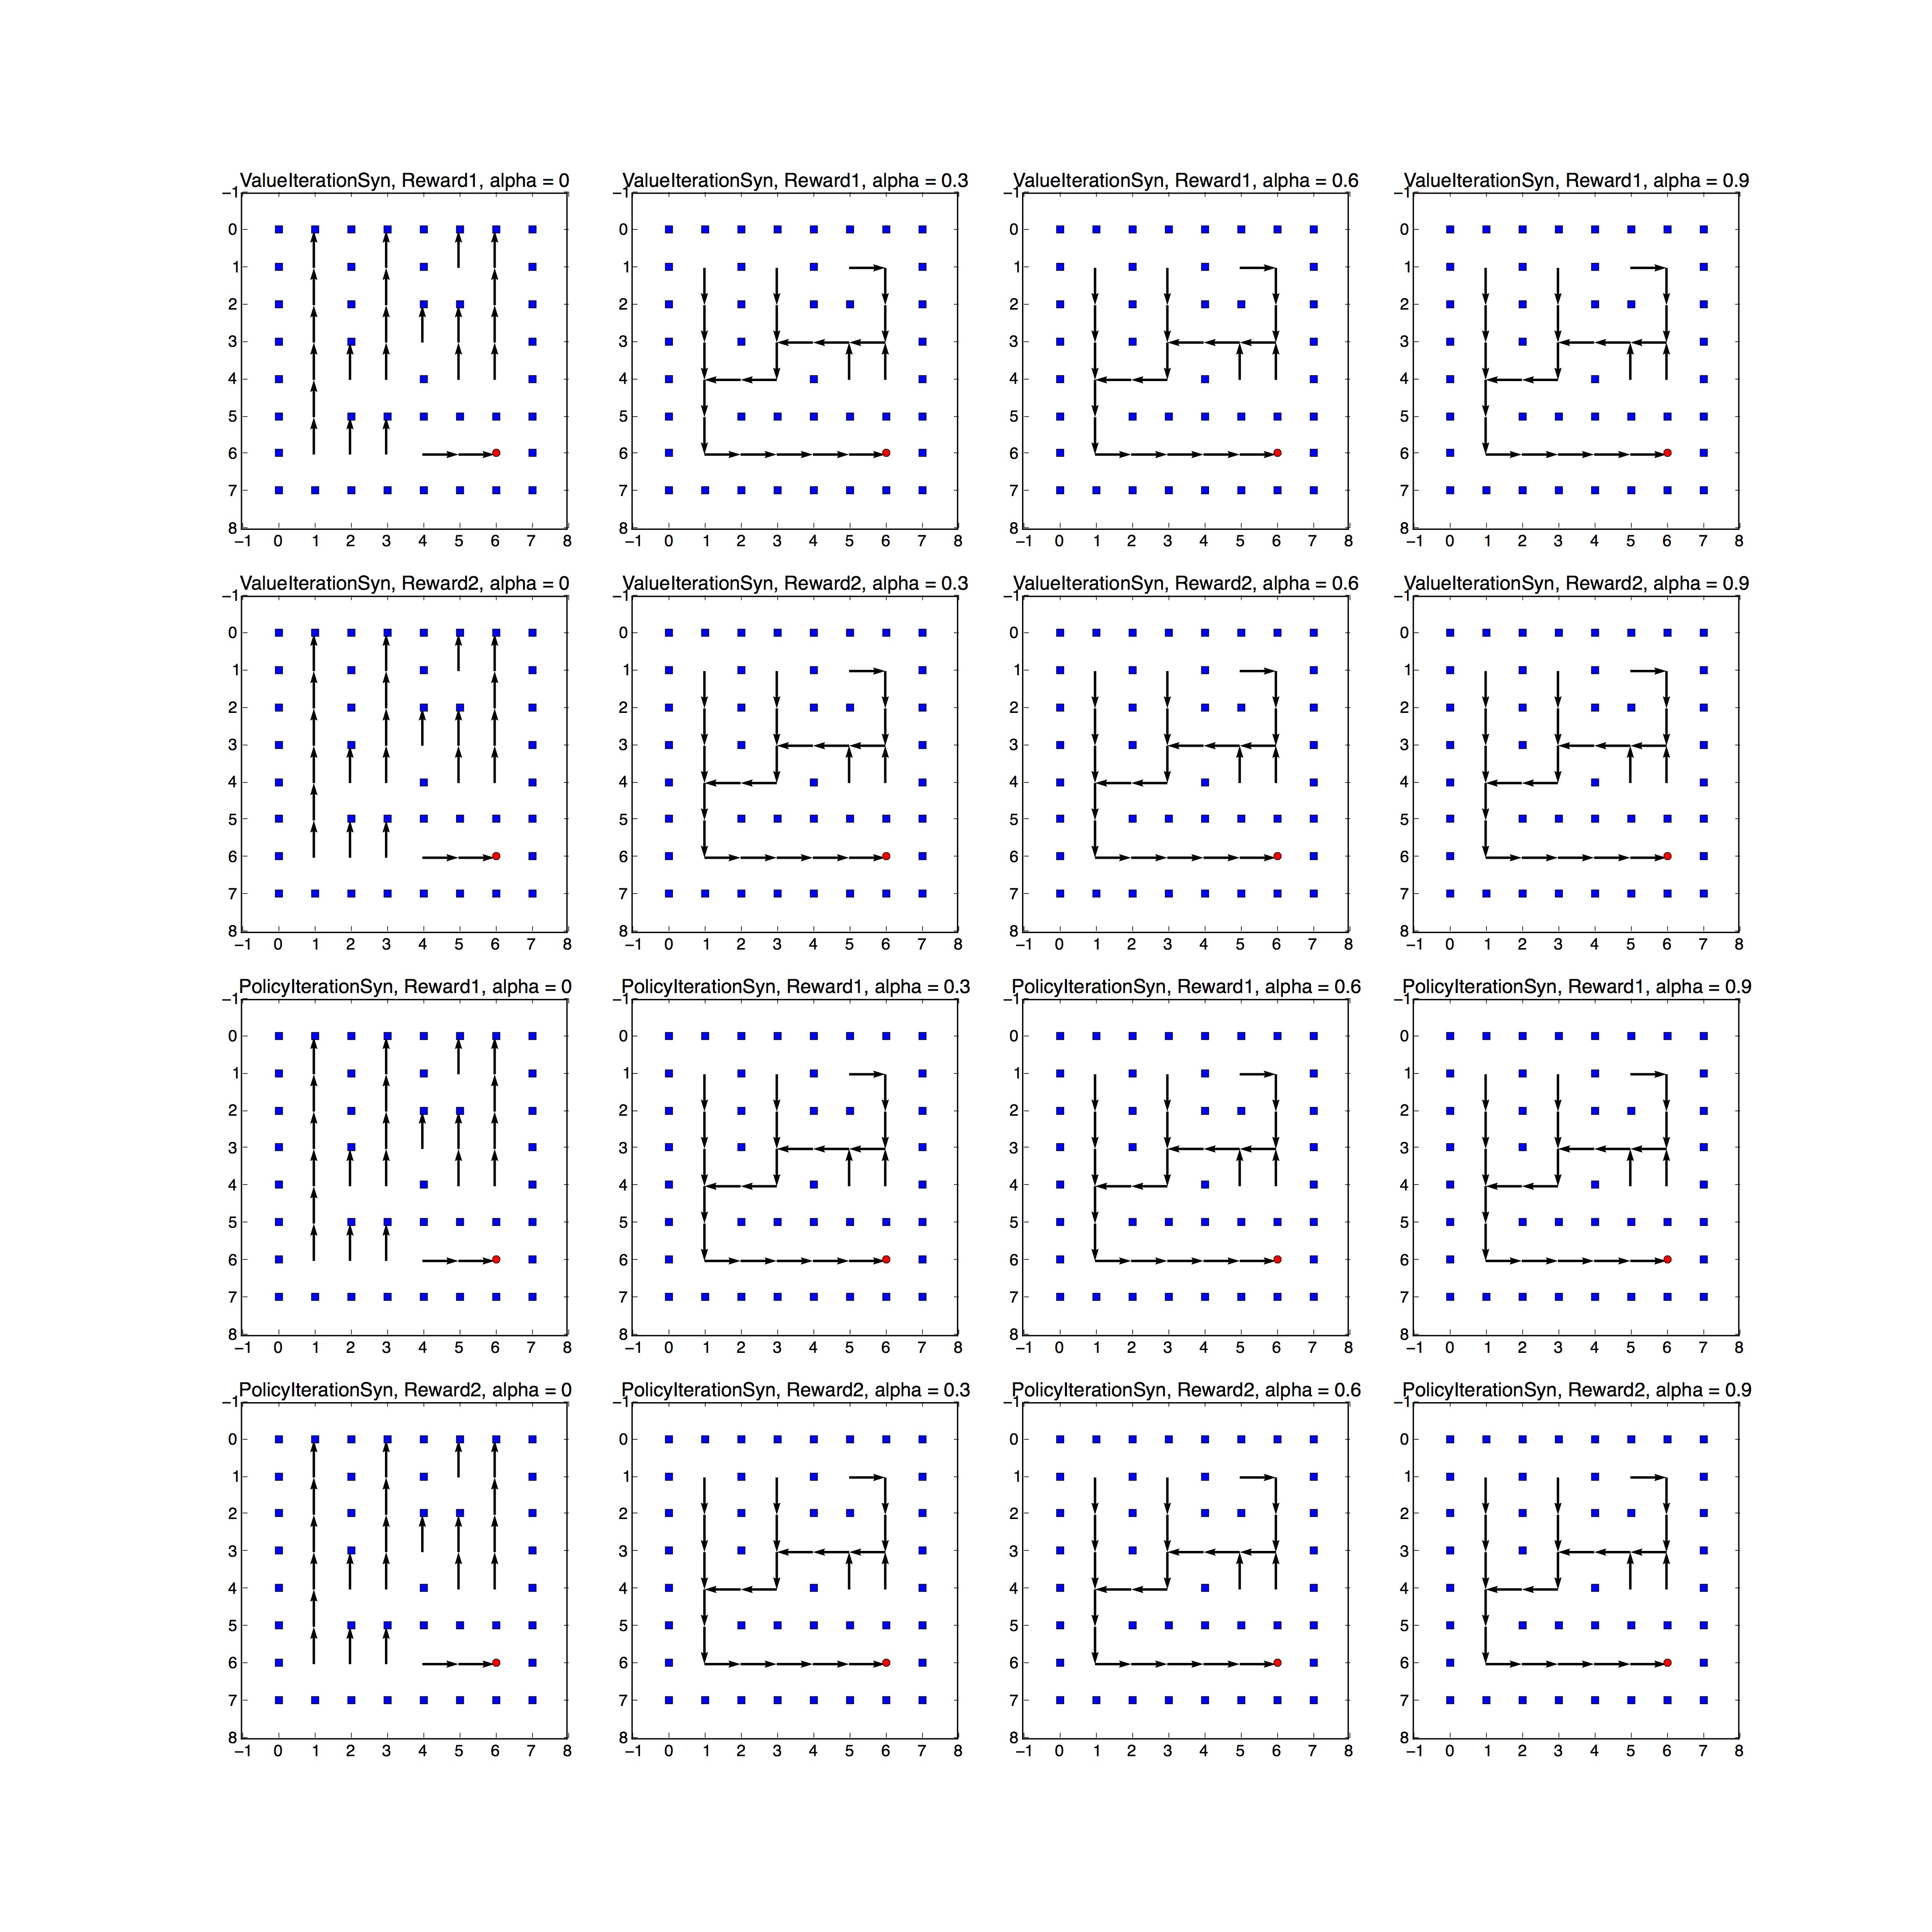
\includegraphics[scale=0.11]{PolicyPlot.jpg}
\end{center}
\newpage
\subsection*{2. Error plots according to different parameter setting}
\begin{center}
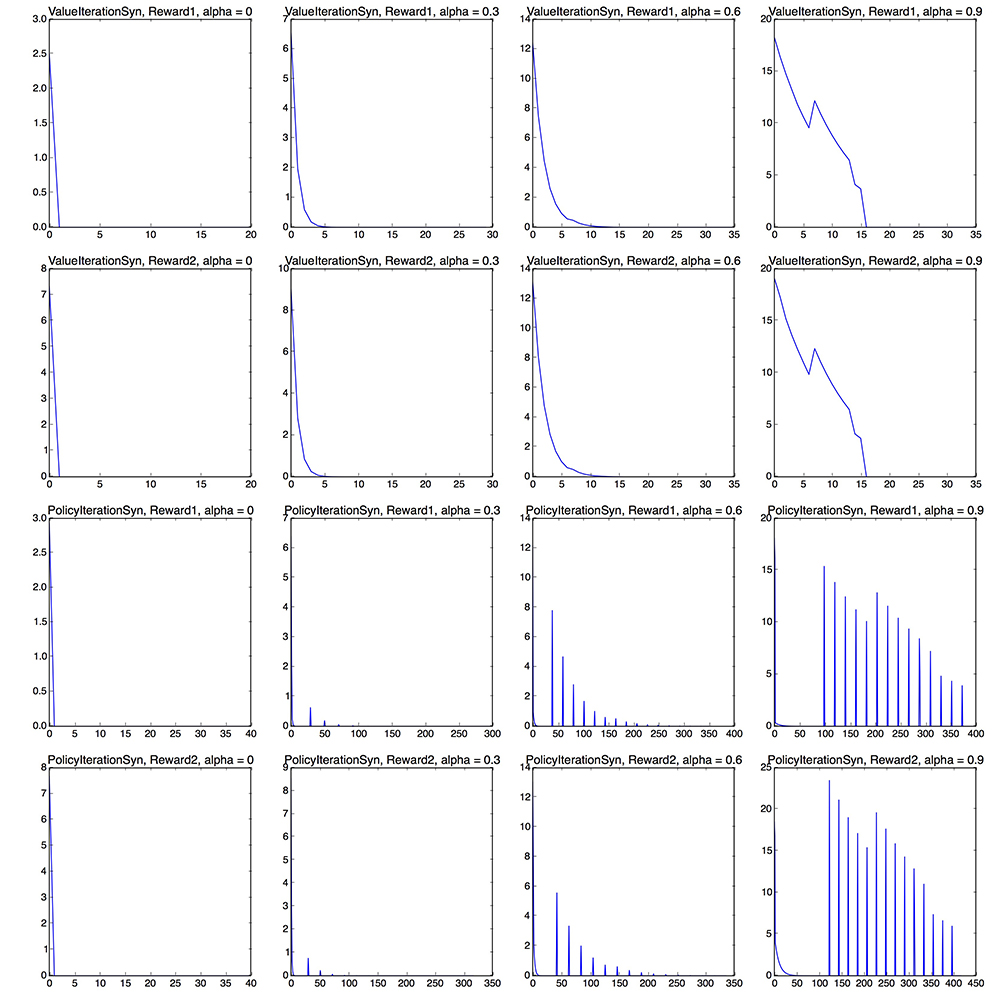
\includegraphics[scale=0.11]{ErrorPlot.jpg}
\end{center}
\newpage
\subsection*{3. MSE To Ground Truth}
\begin{center}
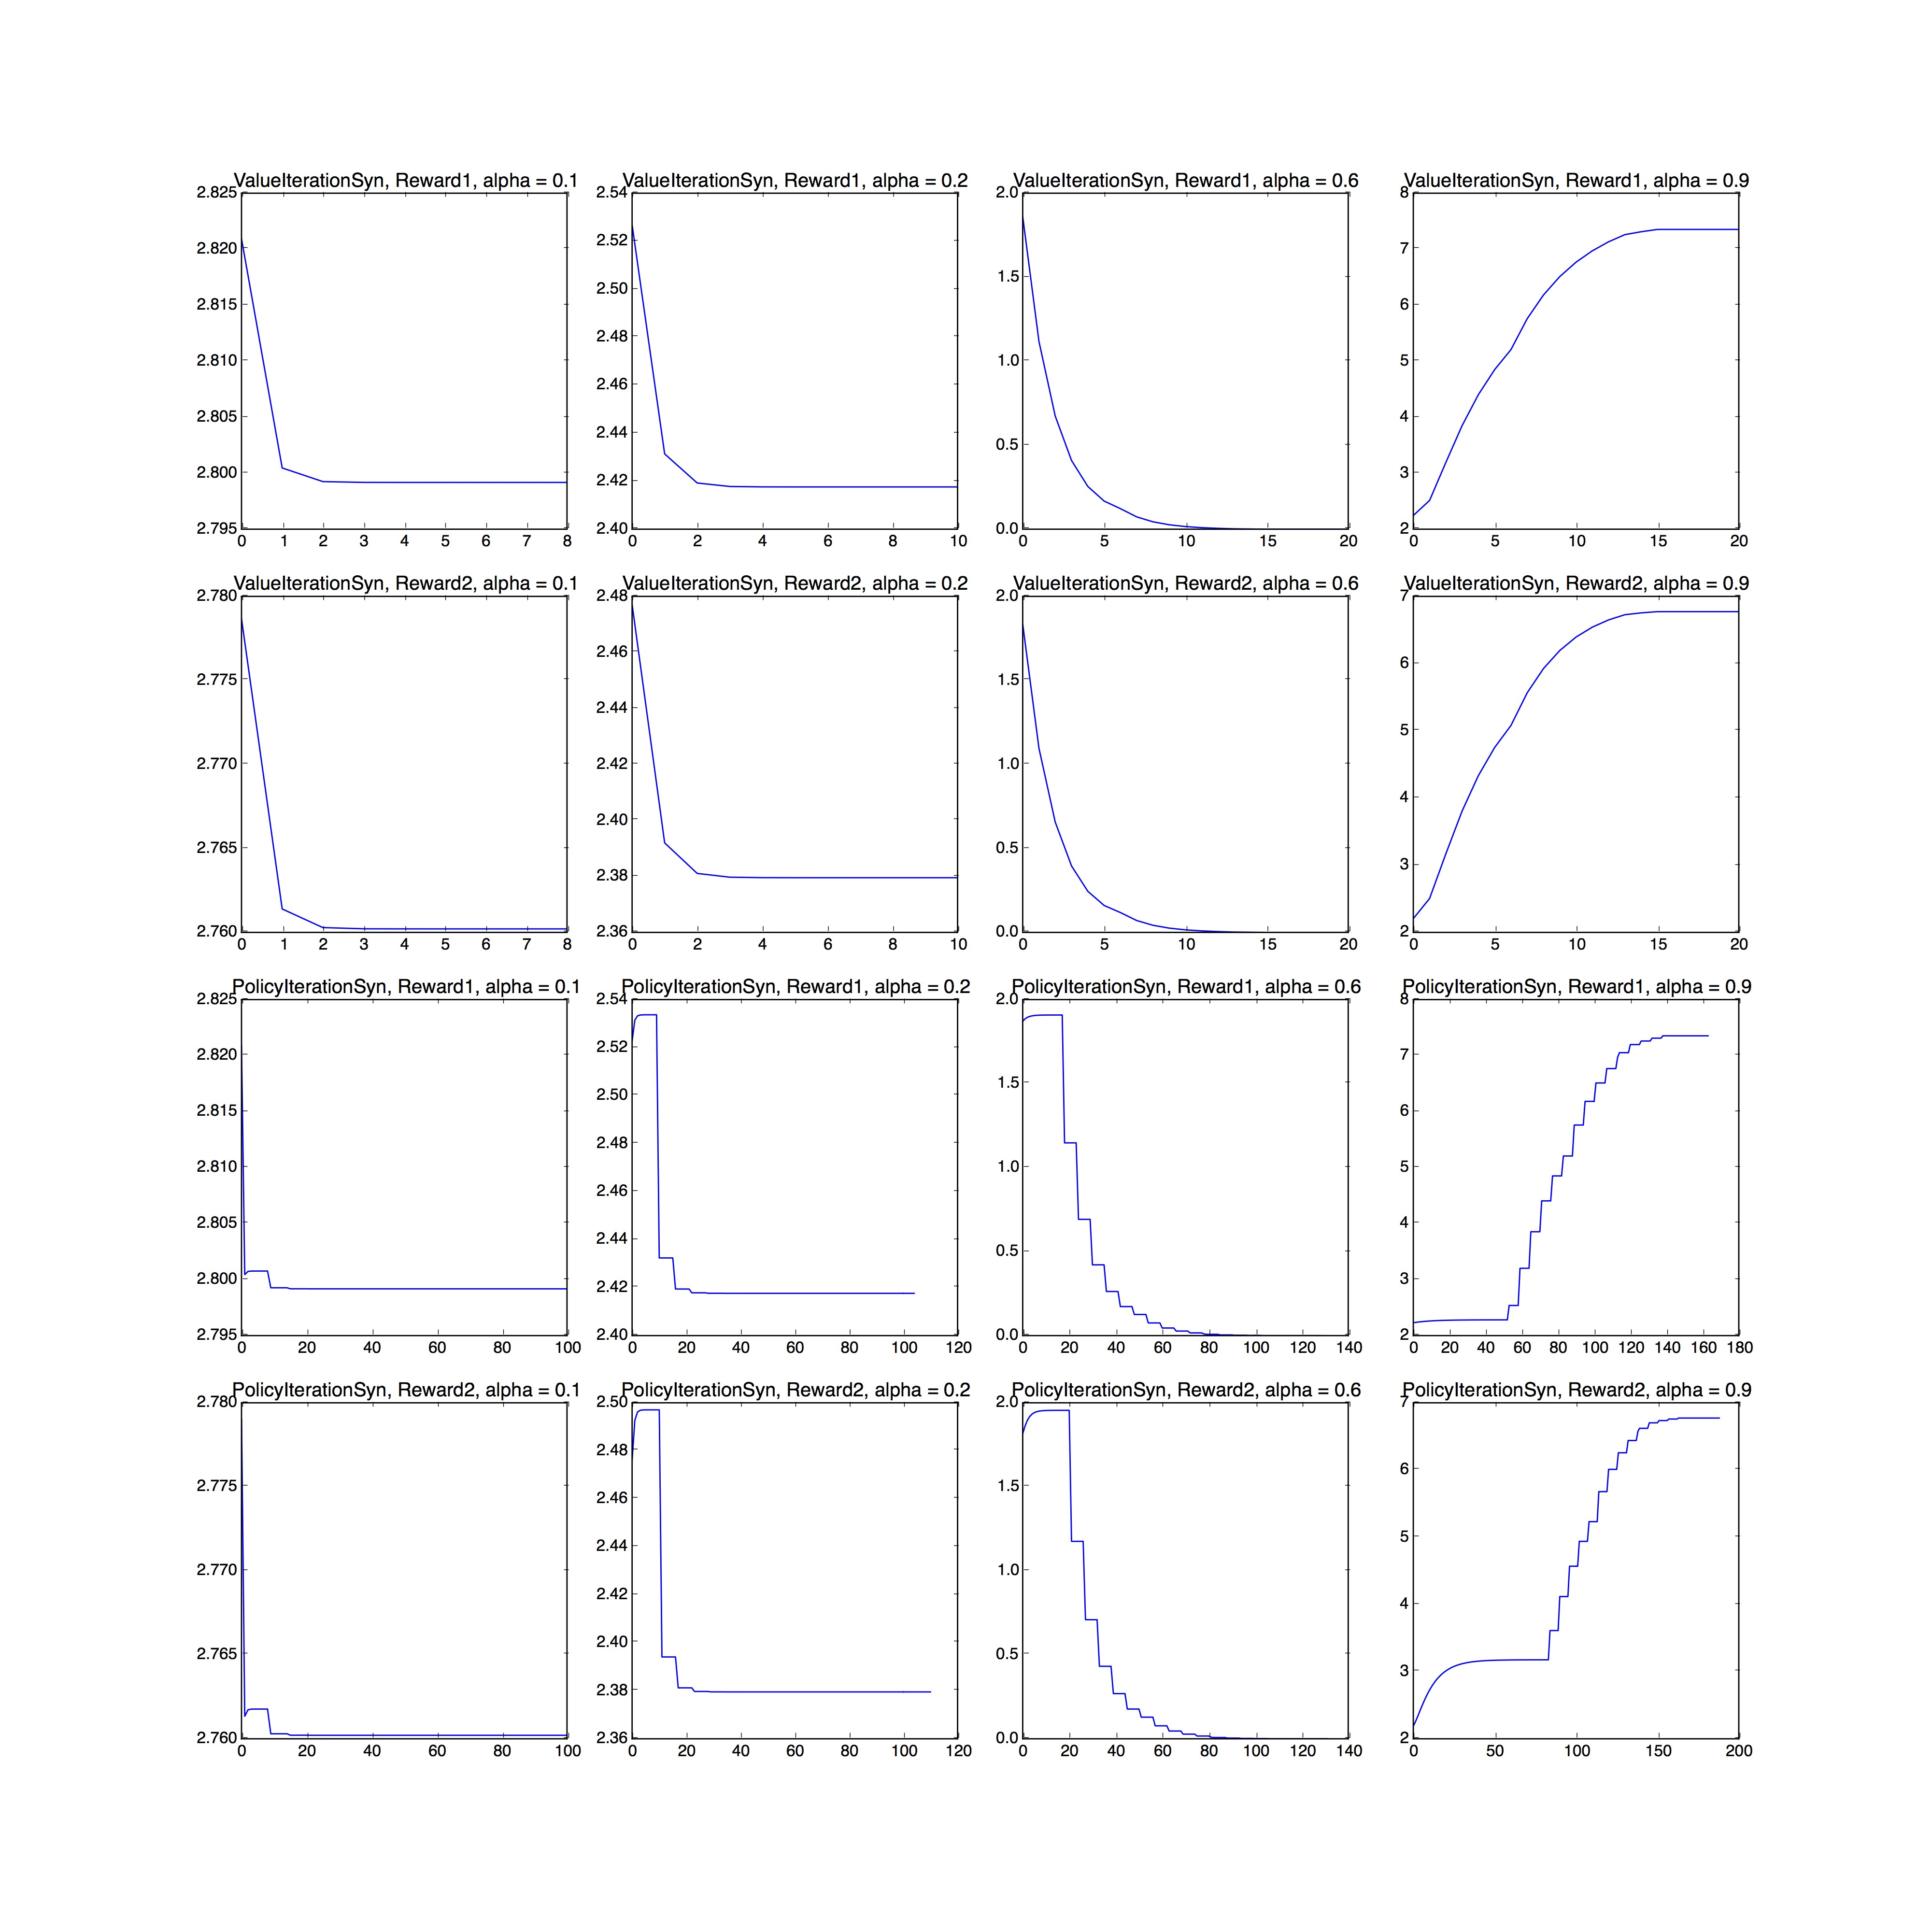
\includegraphics[scale=0.11]{ErrorToGroundTruth.jpg}
\end{center}
\newpage
\subsection*{4. Value function plots according to different parameter setting}
\begin{center}
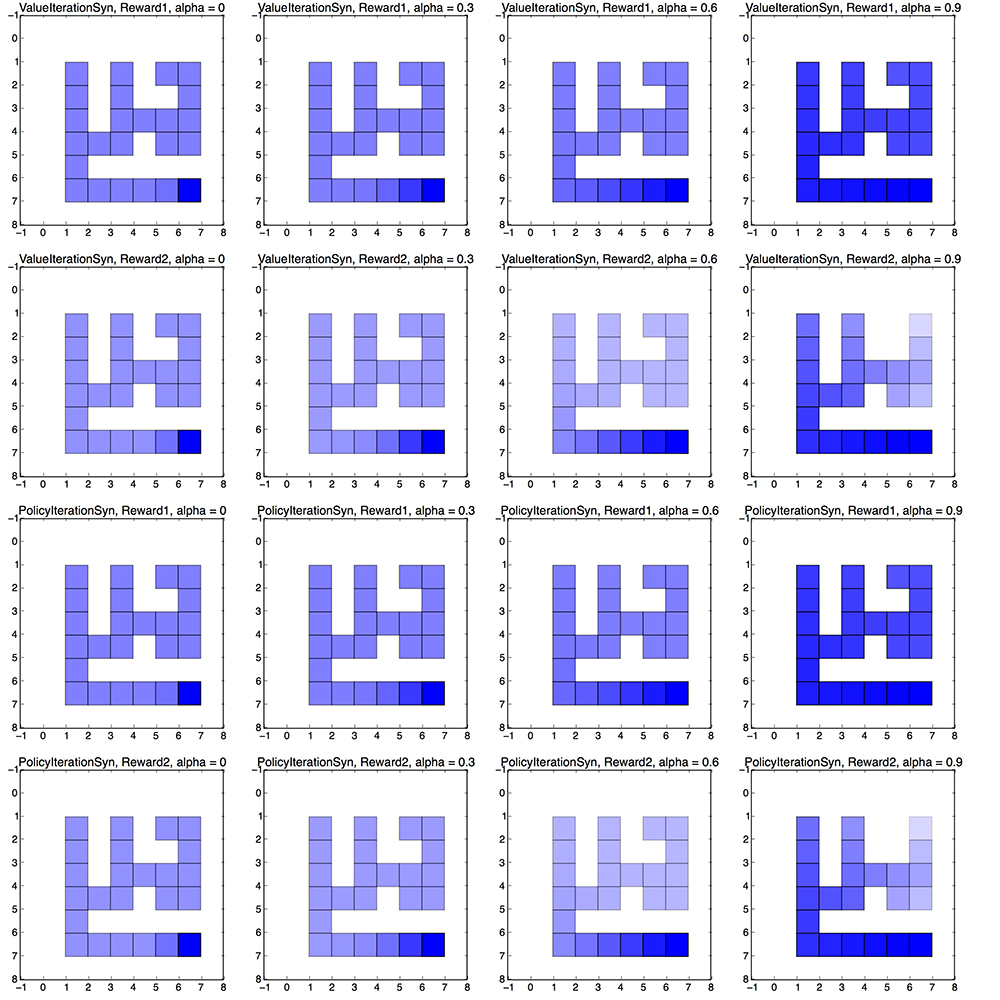
\includegraphics[scale=0.11]{ValueFunctionPlot.jpg}
\end{center}
\end{document}
